\sectionn{Identification and Strategies}

Due to the lack of an official definition for order blocks, traders have developed their own definitions while analyzing these areas on price structures. Some prefer to define a series of horizontal blocks as an OB zone, while others consider the last candle before an impulsive move, with or without the candle wicks, as the OB zone. In my opinion, rather than strictly adhering to any of these definitions, it is necessary to filter the definition on the relevant instrument and select the most appropriate one based on back-testing results. Although I do not yet have a numerical measurement, according to some filters obtained through empirical methods, the identification techniques that will be discussed throughout the report yield effective results.

Since institutions aiming to influence the trend do not trade in micro timeframes, OB zones should first be sought in swing zones formed in higher timeframes (1D and 4H). Then, by descending to micro timeframes (15m), an OB structure should be sought again within the OB zone identified in the higher timeframe. Generally, wicks are excluded in OBs sought in higher timeframes, whereas they are included in candles sought in micro timeframes. If the OB zone determined by including the wicks covers a wide area, applying Fibonacci within this zone can help find a more optimal entry level. Furthermore, since institutions are expected to gradually enter their orders to better manage their average trade prices and then make a move that influences the trend by pushing the price in the direction of their expectations, it is preferable that the candle formed after the order block candle is a voluminous, sharp, and imbalance-creating candle. Additionally, opportunities exist in order blocks that have not yet been mitigated (i.e. fresh order blocks); otherwise, the risk begins to increase. (see: Fig 1).

\begin{figure}[h]
    \centering
    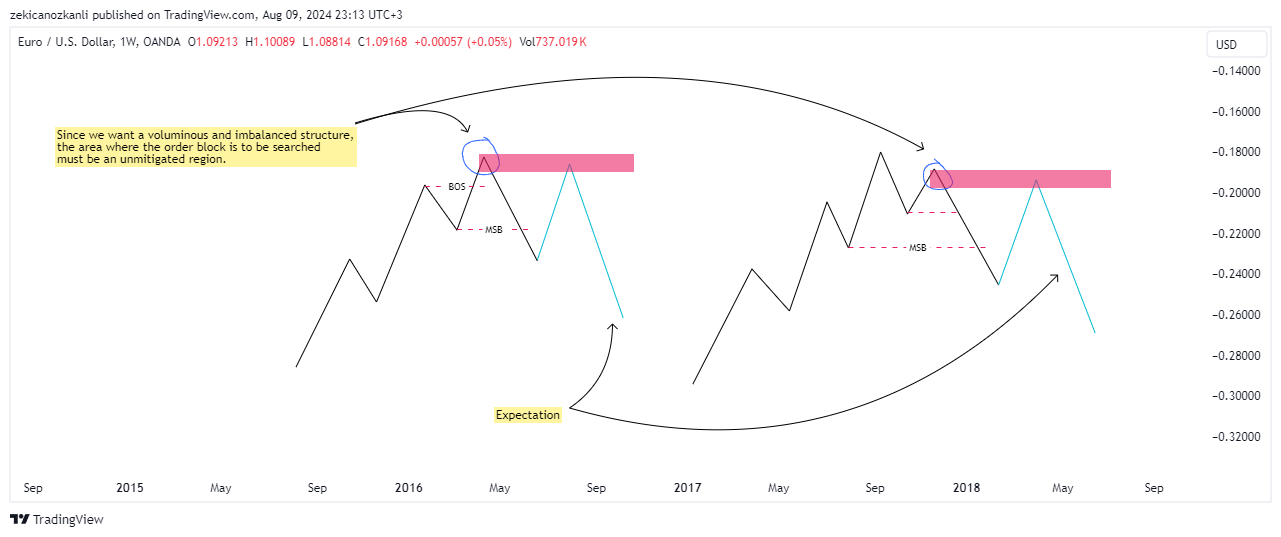
\includegraphics[scale=0.35]{Images/OB-1.png}
    \caption{}
    \label{Fig.1}
\end{figure}

For bullish order blocks, the high and low levels of the order block candle should be below the close and low levels of the subsequent impulsive candle, respectively. For bearish order blocks, the low and high levels of the order block candle should be above the close and high levels of the impulsive candle that follows, respectively. Additionally, while the color of the candle preceding the order block candle is not significant, there are traders who argue that there should be opposite colors between the order block candle and the impulsive candle. However, the general consensus does not support this second piece of information (see: Fig 2). In summary, among the most important factors to consider when identifying an order block are that the order block candle should have taken liquidity, the subsequent candle should be impulsive, and there should be an imbalance between the order block and the impulsive candle. Some examples are shown in Fig 3 and Fig 4. \cite{OB1} \cite{OB2}.

\begin{figure}[H]
    \centering
    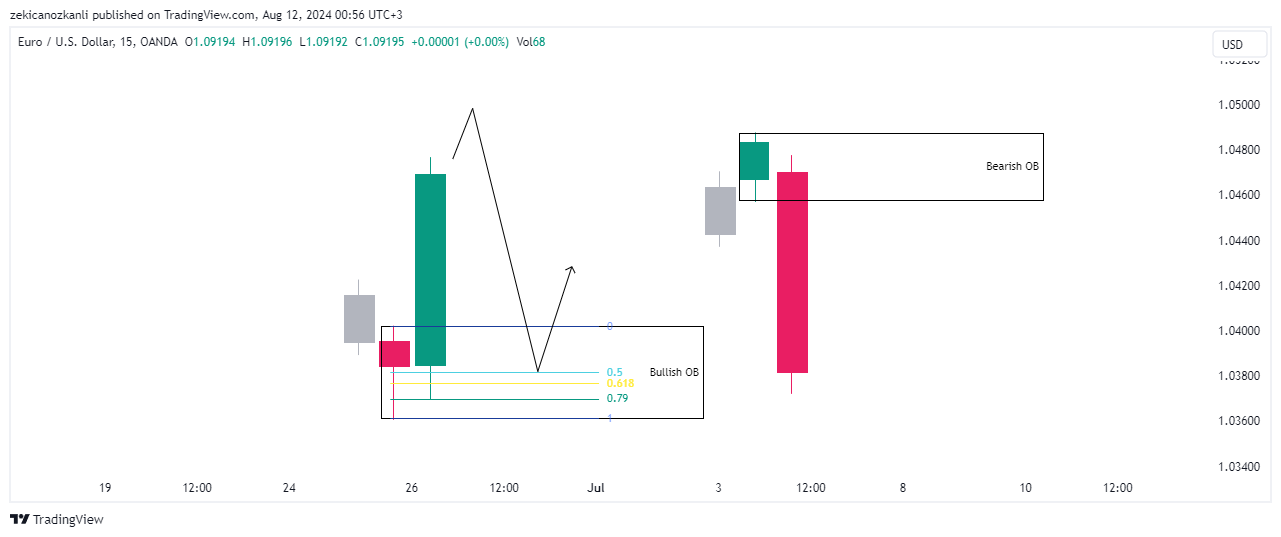
\includegraphics[scale=0.35]{Images/OB-2.png}
    \caption{}
    \label{Fig.2}
\end{figure}

\begin{figure}[H]
    \centering
    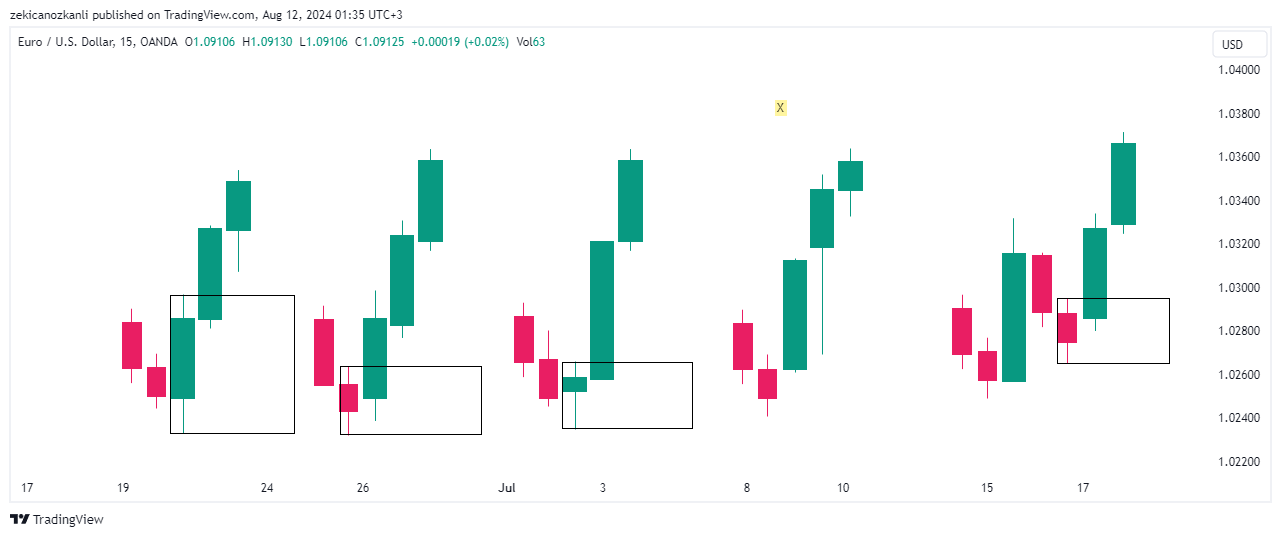
\includegraphics[scale=0.35]{Images/OB-3.png}
    \caption{}
    \label{Fig.3}
\end{figure}
\begin{figure}[H]
    \centering
    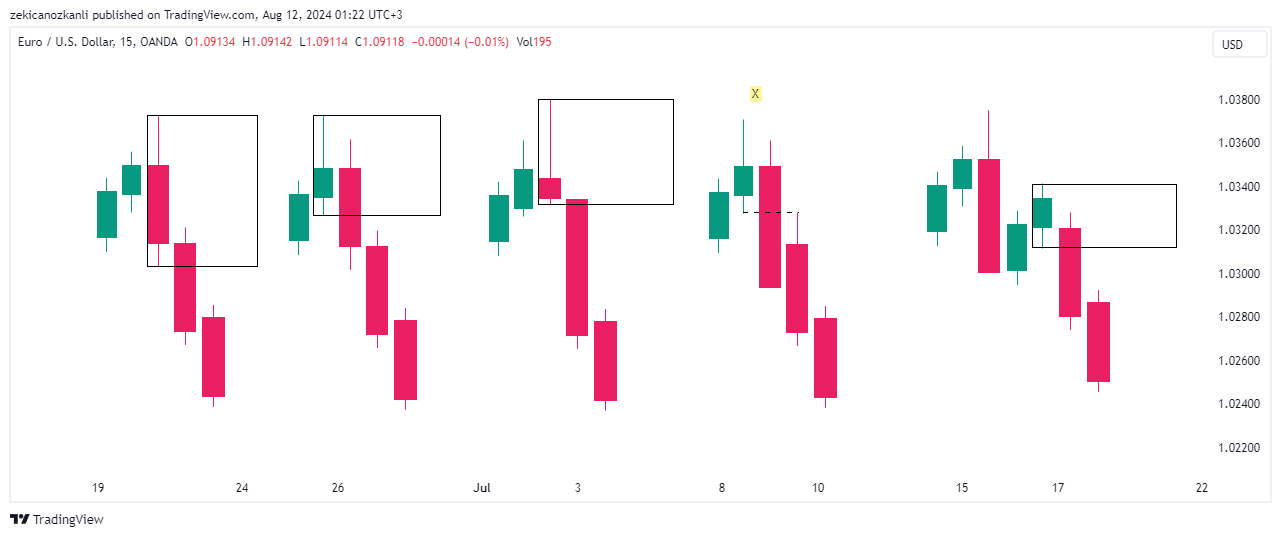
\includegraphics[scale=0.35]{Images/OB-4.png}
    \caption{}
    \label{Fig.4}
\end{figure}
